\documentclass[11pt, a4paper]{article}

\usepackage{graphicx}
\usepackage[a4paper,top=3cm,bottom=2cm,left=2cm,right=2cm,marginparwidth=1.75cm]{geometry}
\usepackage[english]{babel}
\usepackage[utf8x]{inputenc}
\usepackage{subfig}
\usepackage{float}
\usepackage{amsmath}
\usepackage{amssymb}
\usepackage{mhchem}
\usepackage{hyperref}
\usepackage{tikz}
\usepackage{cancel}

\graphicspath{ {./images} }
\newcommand*{\qed}{\hfill\ensuremath{\quad\square}}%
\newcommand*{\rad}{\ensuremath{\,\text{rad}}}
\newcommand*{\R}{\ensuremath{\mathbb{R}}}
\newcommand*{\C}{\ensuremath{\mathbb{C}}}
\renewcommand*{\Re}{\operatorname{Re}}
\renewcommand*{\Im}{\operatorname{Im}}
\renewcommand*{\epsilon}{\varepsilon}
\renewcommand*{\phi}{\varphi}

\makeatletter
\renewcommand*\env@matrix[1][*\c@MaxMatrixCols c]{%
  \hskip -\arraycolsep
  \let\@ifnextchar\new@ifnextchar
  \array{#1}}
\makeatother

\newtheorem{theorem}{Theorem}

%------------------------------------------------
%Templates for images and figures
% \begin{figure}[h]
%   \centering
%   \subfloat[caption 1]{{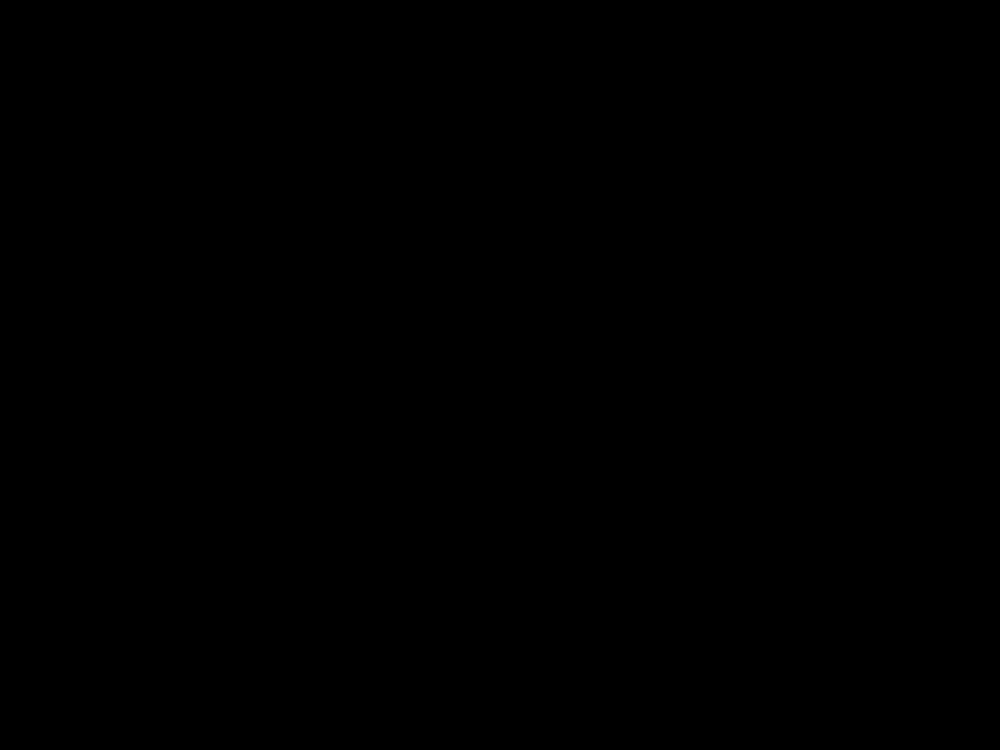
\includegraphics[width=30mm]{images/placeholder.png}}}%
%   \qquad
%   \subfloat[caption 2]{{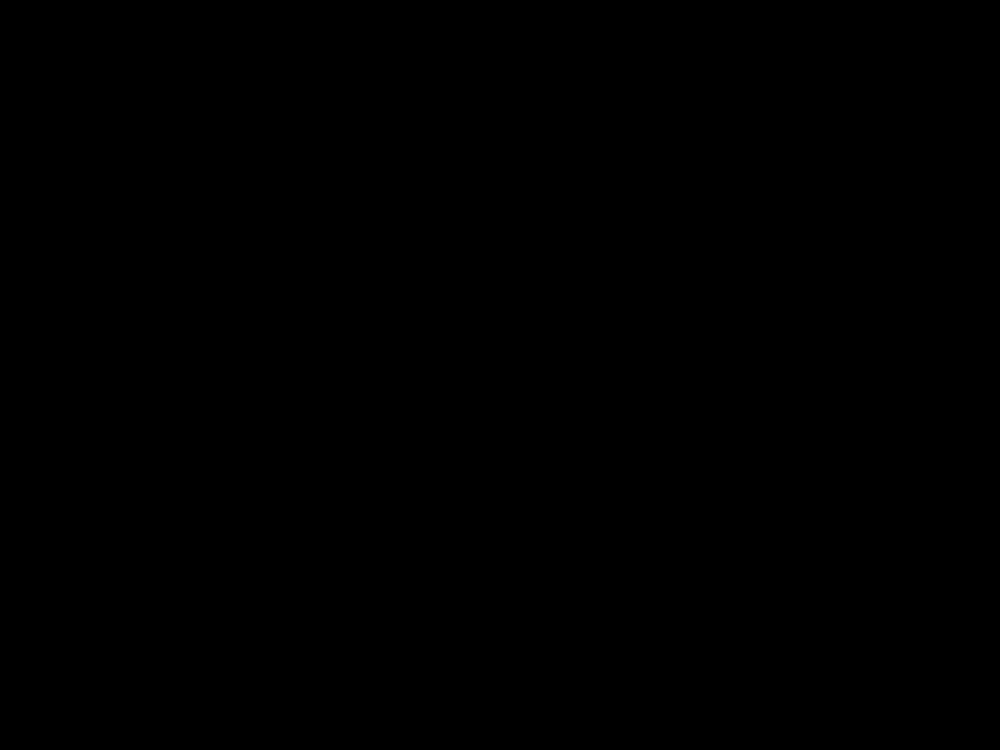
\includegraphics[width=30mm]{images/placeholder.png}}}%
%   \caption{Description}
% \end{figure}

% \begin{figure}[h]
%   \centerline{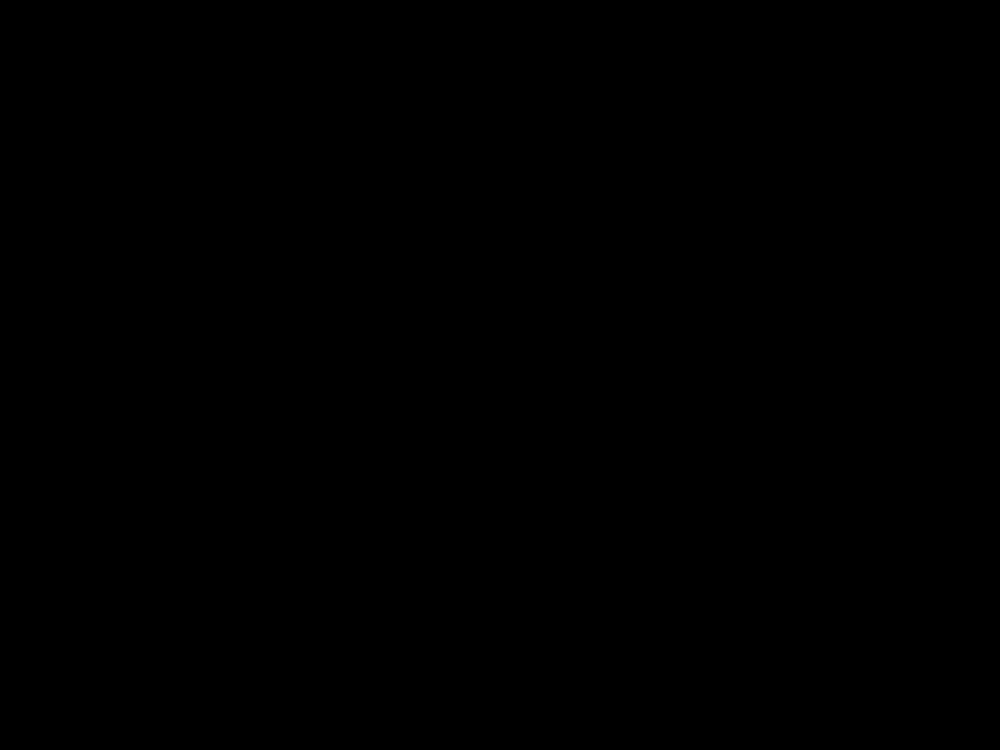
\includegraphics[width=50mm]{images/placeholder.png}}
%   \caption{Description}
% \end{figure}

%Template for a simple table 
%\begin{table}[h]
%   \caption{Description} %title of the table
%   \centering % centering table
%   \begin{tabular}{l rr} % creating three columns
%     \hline\hline %inserting double-line
%     & & \\ [0.5ex] % Insert half line vertical spacing
%     \hline % inserts single-line
%     & & \\ 
%     & & \\
%     & & \\
%     & & \\
%   \hline % inserts single-line
%   \end{tabular}
%   \label{tab:hresult}
% \end{table}
%-----------------------------------------------

\begin{document}
\setcounter{section}{1}
\section{Continuation of introduction to Rigid Body Dynamics}


\subsection{Convention for unit notation}
Units are denoted after the quantity, \underline{not} in square brackets. Square brackets denote an operator which extracts the unit from a physical quantity. Examples of correct notation of units are:
\begin{gather*}
  F = m\cdot \vec{a} = 3\,kg \cdot \vec{a}\\
  [F] = N
\end{gather*}


\subsection{Verification of answers}
Assume the following FBD was given:
\begin{figure}[h]
  \centerline{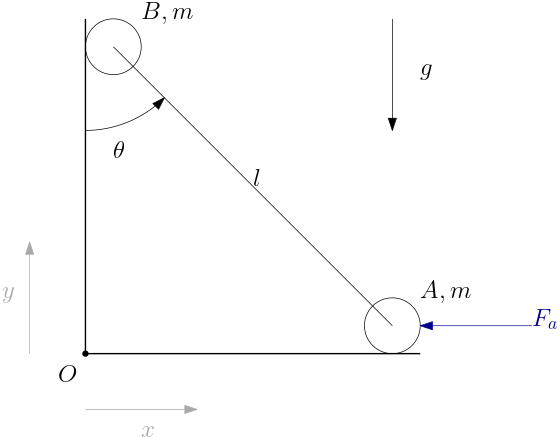
\includegraphics[width=100mm]{images/Sliding_rod.png}}
  \caption{The FBD from which the equation of motion we want to check is derrived}
\end{figure}
Someone has derrived the equation of motion as:
\begin{equation*}
  \ddot{\theta} = \frac{g}{l}\sin(\theta) - \frac{F_a}{m\cdot l}\cos(\theta)
\end{equation*}
We want to quickly verify whether this is correct, without derriving the EoM ourselves. The first check we can do is assume a special case for which the expected answer is easy to predict. Let's look at the case where $\theta = 0\rad$. In this case we also assume $F_a = 0\,N$. Because of this we also expect the value for $\ddot{\theta}$ to be $0$ as the ladder will stand upright against the wall. Filling this in we get:
\begin{equation*}
  \ddot{\theta} = \frac{g}{l}\sin(0\,rad) - \frac{0\,N}{m\cdot l}\cos(0\rad) = 0\rad/s^2
\end{equation*}
Which checks out with our expectation. As a different type of verification we can also use static equilibrium to find a relation between $F_a$ and the angle $\theta$. This works because the relation between $F_a$ and $\theta$ should be the same in both static and dynamic situations. The expression according to statics works out as:
\begin{equation*}
  F_a = \frac{1}{2}g\tan(\theta)
\end{equation*}
If we find the same relation between $F_a$ and $\theta$ we can assume our relation is correct.\\
Furthermore we can use dimensional analysis as a quick check.
\begin{align*}
  [\ddot{\theta}]  &= \frac{[g]}{[l]}[\sin(\theta)] - \frac{[F_a]}{[m]\cdot [l]}[\cos(\theta)]\\
  \frac{\rad}{s^2} &= \frac{\cancel{m}/s^2}{\cancel{m}} \cdot 1 - \frac{\cancel{kg}\cdot \cancel{m}/s^2}{\cancel{kg}\cdot \cancel{m}} \cdot 1\\
  \frac{\rad}{s^2} &= \frac{1}{s^2} - \frac{1}{s^2}
\end{align*}
Which checks out because $1\rad = 1 \frac{m}{m} = 1$.


\subsection{The eqiopllence principle}
An equipollent system of force and torque resultants has the same effect on a rigid body as the original system of forces and torques. The equipollent system with all the forces and moments situated at some point $O$ can be found using:
\begin{align*}
  \vec{F}_r &= \sum_{i=1}^{N} \vec{F}_i\\
  \vec{M}_r &= \sum_{j=1}^{k} \vec{M}_j + \sum_{i=1}^{N} \vec{r}_i \times \vec{F}_i
\end{align*}


\end{document}